%!TEX root = thesis.tex
%-------------------------------------------------------------------------------
\chapter{On the properties of the extended nonlocal game model}
\label{chap:infinite_entanglement}
%-------------------------------------------------------------------------------

This chapter is focused on studying the relationship between \emph{quantum-classical games} and extended nonlocal games. In Section~\ref{sec:quantum-classical-games}, we formally define the model of quantum-classical games, which is a variant of an ordinary nonlocal game, where now, in this model, the referee sends quantum registers to Alice and Bob in place of sending classical messages. This variant was considered by Buscemi~\cite{Buscemi2012} under the name of \emph{semi-quantum games}, and was also considered by Regev and Vidick~\cite{Regev2013}, where they studied a class of quantum-classical games, referred to as \emph{quantum XOR games}, where the winning condition is predicated upon an XOR function. 

One of the main results of Regev and Vidick's paper was to show that there exists a class of quantum XOR games for which no finite-dimensional quantum strategy can be optimal. In Section~\ref{sec:constructing-extended-nonlocal-games-from-quantum-classical-games}, we analyze this result in the context of extended nonlocal games, and building on their framework, show that there also exists a class of extended nonlocal games where no finite-dimensional quantum strategy can be optimal. We then use the relationship between extended nonlocal games and tripartite steering to arrive at the result that there exists a tripartite steering inequality for which an infinite-dimensional quantum state is required in order to achieve a maximal violation. From this, we conclude that there exists extended nonlocal games for which no finite-dimensional standard quantum strategy can be optimal. 

Finally, in Section~\ref{sec:variations-on-enlg}, we consider variants on the extended nonlocal game model. As we have covered, an extended nonlocal game is composed of three rounds of communication; where the type of communication in the first round from Alice and Bob to the referee is quantum, and the remaining two question and answer rounds are composed of classical communication. We ask here what happens if we exchange the type of communication for certain rounds and investigate these variations on the extended nonlocal game model. 

This chapter is based on joint work with John Watrous in~\cite{Russo2016}.

\minitoc

%-------------------------------------------------------------------------------
\section{Quantum-classical games}  \label{sec:quantum-classical-games}
%-------------------------------------------------------------------------------

\index{quantum-classical games (QC games)}{\emph{Quantum-classical games}} or \emph{QC games} for short, differ from nonlocal games in that the referee begins the game by preparing a tripartite quantum state and sends one part of it to each player, keeping a part of the state for itself. (This step replaces the generation of a classical question pair $(x,y)$ in an ordinary nonlocal game.) Once the players receive their portion of the tripartite state in a QC game, the players respond with classical answers $a$ and $b$ (as they would in a nonlocal game as well), and finally the referee determines whether the players win or lose by measuring its part of the original quantum state it initially prepared. (This step replaces the evaluation of a predicate $V(a,b|x,y)$ in an ordinary nonlocal game.) Games of this form, with slight variations from the general class just described, were considered by Buscemi~\cite{Buscemi2012} and Regev and Vidick~\cite{Regev2013}. 

Formally, a quantum-classical game (QC game) is specified by the following objects:
\begin{itemize}
	\item A state $\rho \in \Density(\X \otimes \S \otimes \Y)$ of a triple of registers $(\reg{X},\reg{S},\reg{Y})$.
	\item A collection of measurement operators $\{ Q_{a,b} : a \in \GammaA, \ b \in \GammaB \} \subset \Pos(\S)$, for alphabets $\GammaA$ and $\GammaB$.  
\end{itemize}
Viewing a QC game from the referee's perspective, it is played in the following manner:
\begin{enumerate}
	\item The referee prepares $(\reg{X},\reg{S},\reg{Y})$ in the state $\rho$, then sends $\reg{X}$ to Alice and $\reg{Y}$ to Bob. 
	\item Alice responds with $a \in \GammaA$ and Bob responds with $b \in \GammaB$. 
	\item The referee measures $\reg{S}$ with respect to the binary-valued measurement 
		\begin{align}
			\{Q_{a,b}, \I - Q_{a,b}\}.
		\end{align} 
	The outcome corresponding to the measurement operator $Q_{a,b}$ indicates that Alice and Bob \emph{win}, while the other measurement result indicates that they \emph{lose}. 
\end{enumerate}

\begin{figure}[!htpb] 
	\begin{center}
		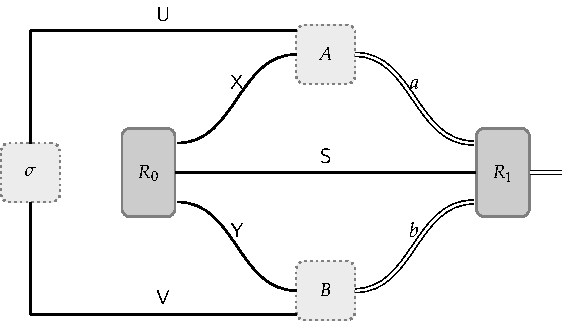
\includegraphics[scale=1.0]{figures/quantum_classical_game.pdf}
	\end{center}
		\caption[A quantum strategy for a quantum-classical game.]{A quantum strategy for a quantum-classical game. Just as in a nonlocal game, if Alice and Bob are using a quantum strategy, they may prepare a state $\sigma \in \Density(\U \otimes \V)$ prior to the start of the game. Unlike a nonlocal game where the referee sends classical information, the referee in a quantum-classical game prepares a state $\rho \in \Density(\X \otimes \S \otimes \Y)$ in registers $(\reg{X},\reg{S},\reg{Y})$ and sends registers $\reg{X}$ and $\reg{Y}$ to Alice and Bob. Alice and Bob perform measurements to generate their answers $a \in \GammaA$ and $b \in \GammaB$, which are then sent back to the referee. The referee then evaluates whether or not Alice and Bob win or lose by making a measurement on its register $\reg{S}$.}
		\label{fig:quantum-classical-game}
\end{figure}

Just as there are various strategies that one may consider for the class of extended nonlocal games, one may also consider various classes of strategies for QC games. We will, however, restrict our attention to \index{quantum strategies (QC games)}{\emph{quantum strategies}} for a QC game. That is, a strategy that consists of a shared quantum state between Alice and Bob, as well as respective sets of measurement operators for Alice and Bob. This type of strategy is similar to a quantum strategy for a nonlocal game, but where now we take into account the fact that the questions that Alice and Bob receive in a QC game are provided via quantum registers. 

More precisely, a quantum strategy for a QC game specified by 
\begin{align}
	\rho \in \Density(\X \otimes \S \otimes \Y)	\quad \textnormal{and} \quad \{Q_{a,b} : a \in \GammaA \ b \in \GammaB \} \subset \Pos(\S)
\end{align}
as above, consists of the following objects:
\begin{enumerate}
	\item A state $\sigma \in \Density(\U \otimes \V)$, for $\U$ being the space corresponding to a register $\reg{U}$ held by Alice and $\V$ being the space corresponding to a register $\reg{V}$ held by Bob. 
	\item A measurement $\{A_a : a \in \GammaA\} \subset \Pos(\U \otimes \X)$ for Alice, performed on the pair $(\reg{U},\reg{X})$ after she receives $\reg{X}$ from the referee, and a measurement $\{ B_b : b \in \GammaB \} \subset \Pos(\Y \otimes \V)$ for Bob, performed on the pair $(\reg{Y},\reg{V})$ after he receives $\reg{Y}$ from the referee. 
\end{enumerate}
A quantum-classical game where Alice and Bob use a quantum strategy is depicted in Figure~\ref{fig:quantum-classical-game}. 

One may express the winning probability for a QC game when Alice and Bob adopt a quantum strategy as 
\begin{align}
	\sum_{(a,b) \in \GammaA \times \GammaB} \biggip{ A_a \otimes Q_{a,b} \otimes B_b }{W \left( \sigma \otimes \rho \right) W^*},
\end{align}
where $W$ is the unitary operator that corresponds to the natural re-ordering of registers consistent with each of the tensor product operators $A_a \otimes Q_{a,b} \otimes B_b$ (i.e. the permutation $( \reg{U}, \reg{V}, \reg{X}, \reg{S}, \reg{Y} ) \mapsto ( \reg{U}, \reg{X}, \reg{S}, \reg{Y}, \reg{V} )$).
The \index{quantum value (quantum-classical game)}{\emph{quantum value}} of a QC game represents the supremum of the winning probabilities, taken over all quantum strategies. If $G_{qc}$ is the name assigned to a QC game having a specification as above, then we write $\omega^*_N(G_{qc})$ to denote the \emph{maximum} winning probability taken over all quantum strategies for which $\dim(\U) = N = \dim(\V)$, so that the quantum value of $G_{qc}$ is 
\begin{align}
	\omega^*(G_{qc}) = \lim_{N \rightarrow \infty} \omega_N^*(G_{qc}).
\end{align}

Regev and Vidick~\cite{Regev2013} proved that certain QC games have the following peculiar property: if Alice and Bob make use of an entangled state of two finite-dimensional quantum systems, initially shared between them, they can never achieve perfect optimality---it is always possible for them to do better (meaning that they win with a strictly larger probability) using some different shared entangled state on two larger quantum systems. Thus, it is only in the limit, as the local dimensions of their shared entangled states goes to infinity, that they can approach an optimal performance in these specific examples of games. This was previously established for analogues of nonlocal games for which both the questions and answers are quantum~\cite{Leung2013}, and it is an open question to determine if the same property holds for any ordinary nonlocal game, where both the questions and answers must be classical.

In particular, Regev and Vidick considered a specific class of QC games called \index{quantum XOR games}{\emph{quantum XOR games}}, where the winning condition in such a game is predicated on an XOR function. Regev and Vidick showed that there exists a family of quantum XOR games such that if the dimension of Alice and Bob's quantum system, $N$, is finite, then the quantum value will be strictly less than $1$. However, taking the limit as $N$ goes to infinity, the quantum value approaches $1$. A restatement of their result follows. 
\begin{theorem}[Theorem 1.2 of~\cite{Regev2013}] \label{thm:regev-vidick-qcg}
	There exists a quantum-classical game $G_{qc}$ such that 
	\begin{align}
		\omega^*(G_{qc}) = 1,
	\end{align}
and for every positive integer $N$ it holds that 
	\begin{align}
		\omega_N^*(G_{qc}) < 1.
	\end{align}
\end{theorem}

%-------------------------------------------------------------------------------
\section[Constructing extended nonlocal games from quantum-classical games]{Constructing extended nonlocal games \\ from quantum-classical games} \label{sec:constructing-extended-nonlocal-games-from-quantum-classical-games}
%-------------------------------------------------------------------------------

In this section, we will state and prove an analogous theorem to Theorem~\ref{thm:regev-vidick-qcg} for an extended nonlocal game. That is, we will show that there exists an extended nonlocal game where the standard quantum value approaches $1$ when the dimension of the quantum systems shared by Alice and Bob approach infinity. 
\begin{theorem} \label{thm:enlg-from-qcg}
	Given a quantum-classical game, $G_{qc}$ with question registers $\reg{X}$ and $\reg{Y}$, there exists an extended nonlocal game, labelled as $H_t$, such that
	\begin{align} \label{eq:enlg-from-qcg}
		\omega_N^*(G_{qc}) \leq 1 - \abs{\reg{X}} \abs{\reg{Y}} \left( 1- \omega^*_{N \abs{\reg{X}} \abs{\reg{Y}}}(H_t) \right) \quad \textnormal{and} \quad \omega_N^*(H_t) \leq 1 - \frac{ 1 - \omega^*_{N \abs{\reg{X}} \abs{\reg{Y}}}(G_{qc}) }{\abs{\reg{X}} \abs{\reg{Y}}}.
	\end{align}
\end{theorem}
The main idea for proving Theorem~\ref{thm:enlg-from-qcg} will involve a successive reduction from a quantum-classical game to an intermediate type of game, called a \emph{teleportation game} (that we will define formally in the next section), and finally to an extended nonlocal game. Sections~\ref{sec:teleportation-games-and-quantum-classical-games} and~\ref{sec:extended-nonlocal-games-and-teleportation-games} are dedicated to proving Theorem~\ref{thm:enlg-from-qcg}. Specifically, in Section~\ref{sec:teleportation-games-and-quantum-classical-games}, we will show how quantum-classical games are related to teleportation games, and in Section~\ref{sec:extended-nonlocal-games-and-teleportation-games}, we will show how teleportation games are related to extended nonlocal games. Once these relationships are established, we will be able to prove Theorem~\ref{thm:enlg-from-qcg}.

%-------------------------------------------------------------------------------
\subsection{Teleportation games and quantum-classical games} \label{sec:teleportation-games-and-quantum-classical-games}
%-------------------------------------------------------------------------------

In this section we will introduce \index{teleportation game}{\emph{teleportation games}}. A teleportation game is similar to an extended nonlocal game in that the referee receives a state prepared by Alice and Bob, the referee sends questions to Alice and Bob, and the referee receives answers from them as well. The one key difference now is that after the referee receives the state from Alice and Bob, it will produce registers and perform a Bell measurement on the parts of the state sent by Alice and Bob along with the registers that it produced. The reason we refer to this class of games as teleportation games is because the registers that the referee produces are the registers that the referee desires to teleport to Alice and Bob. A teleportation game is depicted in Figure~\ref{fig:teleportation-game}.

Formally, a \emph{teleportation game} is specified by the following objects:
\begin{itemize}
	\item A state $\rho \in \Density(\X \otimes \S \otimes \Y)$ of a triple of registers $(\reg{X},\reg{S},\reg{Y})$. 
	\item A collection of measurement operators $\{ Q_{a,b} : a \in \GammaA, \ b \in \GammaB \} \subset \Pos(\S)$, where $\GammaA$ and $\GammaB$ are alphabets and $\S$ is the space corresponding to register $\reg{S}$. 
\end{itemize}
From the referee's perspective, such a game is played as follows:
\begin{enumerate}
	\item The referee is presented with the register $\reg{R} = (\reg{X}_1,\reg{Y}_1)$ where $\reg{X}_1$ and $\reg{Y}_1$, are copies of the registers $\reg{X}$ and $\reg{Y}$. (The register $\reg{R}$ might, for instance, be entangled with systems possessed by Alice and Bob.)
	\item The referee prepares $(\reg{X},\reg{S},\reg{Y})$ in the state $\rho$ and performs Bell measurements
		\begin{align} \label{eq:bell-basis-telep-game}
			\left \{ \phi_{x}^{(\abs{\reg{X}})} : x \in \SigmaA \right \} \subset \Pos(\X \otimes \X_1) \quad \textnormal{and} \quad \left \{ \phi_{y}^{(\abs{\reg{Y}})} : y \in \SigmaB \right \} \subset \Pos(\Y \otimes \Y_1)
		\end{align}		
	 and where 
	\begin{align}
	 	\SigmaA = \integer_{\abs{\reg{X}}} \times \integer_{\abs{\reg{X}}} \quad \textnormal{and} \quad \SigmaB = \integer_{\abs{\reg{Y}}} \times \integer_{\abs{\reg{Y}}},
	 \end{align}
	 on the respective pairs $(\reg{X},\reg{X}_1)$ and $(\reg{Y},\reg{Y}_1)$ yielding outcomes $x \in \SigmaA$ and $y \in \SigmaB$ which are sent to Alice and Bob.
	\item Alice and Bob respond with $a \in \GammaA$ and $b \in \GammaB$. 
	\item The referee measures $\reg{S}$ with respect to the binary-valued measurement 
		\begin{align}
			\{Q_{a,b}, \I - Q_{a,b}\} \subset \Pos(\S).		
		\end{align} 
	The outcome corresponding to the measurement operator $Q_{a,b}$ indicates that Alice and Bob \emph{win}, while the other measurement result indicates that they \emph{lose}.  
\end{enumerate}

Just as is the case for both extended nonlocal games and quantum-classical games, one may consider various types of strategies for Alice and Bob. For the purposes of this discussion, we will be focusing on \index{quantum strategy (teleportation game)}{\emph{quantum strategies}} in which Alice and Bob begin the game in possession of finite-dimensional quantum systems that have been initialized as they choose. They may then measure these systems in order to obtain answers to the referee's questions. 

In more precise terms, a quantum strategy for a teleportation game, specified by 
	\begin{align}
		\rho \in \Density(\X \otimes \S \otimes \Y) \quad \textnormal{and} \quad \{Q_{a,b} : a \in \GammaA, \ b \in \GammaB \} \subset \Pos(\S)
	\end{align}
as above, consists of these objects:
\begin{enumerate}
	\item A state $\sigma \in \Density(\U \otimes (\X_1 \otimes \Y_1) \otimes \V)$ where $(\X_1 \otimes \Y_1)$ is the space corresponding to registers $(\reg{X}_1, \reg{Y}_1)$ presented to the referee at the start of the game, where $\U$ is the space corresponding to register $\reg{U}$ held by Alice, and where $\V$ is the space corresponding to register $\reg{V}$ held by Bob.
	\item A measurement $\{A_a^x : a \in \GammaA\} \subset \Pos(\U)$ for each $x \in \SigmaA$, performed by Alice, when she receives the question $x$, and a measurement $\{B_b^y : b \in \GammaB\} \subset \Pos(\V)$ for each $y \in \SigmaB$, performed by Bob when he receives the question $y$. 
\end{enumerate}

%When Alice and Bob utilize such a strategy, their winning probability may be expressed as 
%\begin{align}
%	  \sum_{\substack{
%      (x,y) \in \SigmaA \times \SigmaB \\
%      (a,b) \in \GammaA \times \GammaB \\
%  }}
%	\biggip{A^x_a \otimes Q_{a,b} \otimes B^y_b}{ W \left( (\phi_{x}^{(\mA)} \otimes \phi_{y}^{(\mB)}) (\rho \otimes \sigma) (\phi_{x}^{(\mA)} \otimes \phi_{y}^{(\mB)})^* \right) W^* },
%\end{align}
%where the sets of measurements
%\begin{align}
%	\left \{ \phi_{x}^{(\mA)} : x \in \integer_{\mA} \times \integer_{\mA} \right \} \quad \textnormal{and} \quad \left \{ \phi_y^{(\mB)} : y \in \integer_{\mB} \times \integer_{\mB} \right \}
%\end{align}
%correspond to the Bell basis and where $W$ is a unitary operator that corresponds to the natural re-ordering of tensor products. 

If $G_t$ is the name assigned to a teleportation game having the specifications as above, then we write $\omega_N^*(G_t)$ to denote the \emph{maximum} winning probability taken over all quantum strategies for which $\dim(\U \otimes \V) = N$, so that the quantum value of $G_t$ is 
\begin{align}
	\omega^*(G_t) = \lim_{N \rightarrow \infty} \omega_N^*(G_t).
\end{align}

\begin{figure}[!htpb] 
	\begin{center}
		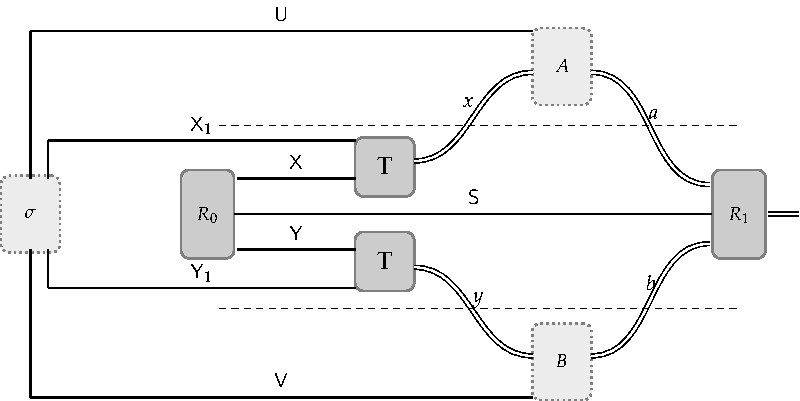
\includegraphics[scale=1.0]{figures/teleportation_game.pdf}
	\end{center}
		\caption[A quantum strategy for a teleportation game.]{A quantum strategy for a teleportation game. Prior to the start of the game, the state $\sigma \in \Density(\U \otimes (\X_1 \otimes \Y_1) \otimes \V)$ is prepared. The referee obtains registers $(\reg{X}_1,\reg{Y}_1)$. The referee prepares a state $\rho \in \Density(\X \otimes \S \otimes \Y)$ contained in registers $(\reg{X},\reg{S},\reg{Y})$ and performs a generalized Bell measurement on registers $(\reg{X},\reg{X}_1)$ and $(\reg{Y},\reg{Y}_1)$. The outcomes of this measurement, $x \in \SigmaA$ is sent to Alice and $y \in \SigmaB$ is sent to Bob, who in turn respond with answers $a \in \GammaA$ and $b \in \GammaB$ to the referee. The referee then performs a measurement on the register $\reg{S}$ to determine whether Alice and Bob win or lose.}
		\label{fig:teleportation-game}
\end{figure}

\begin{lemma} \label{lem:qcg_eq_telep}
	Given any quantum-classical game, $G_{qc}$, with question registers $\reg{X}$ and $\reg{Y}$, there exists a teleportation game $G_t$ such that 
	\begin{align}
		\omega_N^*(G_{qc}) \leq \omega_{N\abs{\reg{X}}\abs{\reg{Y}}}^*(G_t) \quad \textnormal{and} \quad \omega^*_{N}(G_t) \leq \omega^*_{N\abs{\reg{X}}\abs{\reg{Y}}}(G_{qc}),
	\end{align}		
for all $N \geq 1$.
\end{lemma}

Prior to proceeding to the proof, we give a brief sketch to provide some intuition. In order to prove Lemma~\ref{lem:qcg_eq_telep}, we must prove both that $\omega_N^*(G_{qc}) \leq \omega_{N \abs{\reg{X}} \abs{\reg{Y}}}^*(G_t)$ and that $\omega_{N}^*(G_t) \leq \omega_{N\abs{\reg{X}}\abs{\reg{Y}}}^*(G_{qc})$. 

In the first inequality, we assume that Alice and Bob play honestly. That is to say, we assume that Alice and Bob play along and allow the referee to teleport registers to Alice and Bob. For this to happen, the initial state is prepared as a maximally entangled state and Alice and Bob also apply the appropriate Pauli teleportation corrections on their respective systems after they receive the questions from the referee. This direction of the proof is simply illustrating how such a strategy is carried out when Alice and Bob play honestly and is depicted in Figure~\ref{fig:teleportation-game-strategy}. 

In the second inequality, we remove the assumption that Alice and Bob play honestly. That is to say that we are not guaranteed that Alice and Bob prepare maximally entangled states, nor are we to assume that the registers they possess are not entangled in some arbitrarily complex manner. In other words, we are concerned now with the possibility that Alice and Bob may attempt to cheat, and play dishonestly. The general idea of this direction is that Alice and Bob will perform what may be thought of a teleportation protocol to themselves. That is, after Alice and Bob perform measurements in the Bell basis on their registers, they will use the outcome of these measurements to apply the appropriate generalized Pauli correction operator to their systems. 

\begin{proof}
	Let $G_t$ be the teleportation game that is defined in terms of the same state and measurement operators
	\begin{align}
		\rho \in \Density(\X \otimes \S \otimes \Y) \quad \textnormal{and} \quad \{ Q_{a,b} : a \in \GammaA \ b \in \GammaB \} \subset \Pos(\S)
	\end{align}	
that also define $G_{qc}$.  

	Let us first show that $\omega_N^*(G_{qc}) \leq \omega_{N\abs{\reg{X}}\abs{\reg{Y}}}^*(G_t)$. Consider an arbitrary strategy for any quantum-classical game $G_{qc}$. We show how one may adapt this strategy into a strategy for the teleportation game $G_t$. The following strategy is depicted in Figure~\ref{fig:teleportation-game-strategy}
	
	The state $\sigma$ is prepared in the following manner 
	\begin{align}
		\sigma \in \Density( (\U_1 \otimes \X_0) \otimes (\X_1 \otimes \Y_1) \otimes (\Y_0 \otimes \V_1))
	\end{align}		
in registers $(\reg{U}_1, \reg{X}_0, \reg{X}_1,\reg{Y}_1, \reg{Y}_0, \reg{V}_1)$ such that
	\begin{align}
		 \abs{\reg{X}_0} = \abs{\reg{X}} = \abs{\reg{X}_1} \quad \textnormal{and} \quad  \abs{\reg{Y}_0} = \abs{\reg{Y}} = \abs{\reg{Y}_1},	
	\end{align}		
where the contents of $(\reg{X}_0,\reg{X}_1)$ and $(\reg{Y}_0,\reg{Y}_1)$ are respective maximally entangled states 
\begin{align}
	\psi_{\reg{X}} = \frac{1}{\sqrt{\abs{\reg{X}}}} \sum_{c \in \integer_{\abs{\reg{X}}}} e_c \otimes e_c \quad \textnormal{and} \quad \psi_{\reg{Y}} = \frac{1}{\sqrt{\abs{\reg{Y}}}} \sum_{d \in \integer_{\abs{\reg{Y}}}} e_d \otimes e_d.
\end{align}
When the referee receives $\reg{X}_1$ and $\reg{Y}_1$, it prepares the quantum state $\rho \in \Density(\X \otimes \S \otimes \Y)$ contained in registers $(\reg{X},\reg{S},\reg{Y})$.

The referee then measures each pair $(\reg{X},\reg{X}_1)$ and $(\reg{Y},\reg{Y}_1)$ with respect to the Bell basis as from equation~\eqref{eq:bell-basis-telep-game} and obtains outcomes $x$ and $y$, where
\begin{align}
	x = (k_1,k_2) \in \SigmaA \quad \textnormal{and} \quad y = (l_1,l_2) \in \SigmaB,
\end{align}
which are then sent to Alice and Bob. 
%\begin{align} \label{eq:bell-basis-telep-game}
%	\left \{ \phi_{k_1,k_2}^{(\mA)} : k_1, k_2 \in \integer_{\mA} \right \} \quad \textnormal{and} \quad \left \{ \phi_{l_1,l_2}^{(\mB)} : l_1, l_2 \in \integer_{\mB}  \right \}.
%\end{align}
%The outcomes of all measurements on $(\reg{X},\reg{X}_1)$ and $(\reg{Y},\reg{Y}_1)$ are stored in strings as 
%\begin{align}
%	x = (k_1,k_2) \in \integer_{\mA} \times \integer_{\mB} \quad \textnormal{and} \quad y = (l_1,l_2) \in \integer_{\mB} \times \integer_{\mB},
%\end{align}
%where $x \in \SigmaA$ and $y \in \SigmaB$ for alphabets $\SigmaA$ and $\SigmaB$ are sent to Alice and Bob. 
Alice and Bob then apply one of the generalized Pauli operators 
\begin{align} \label{eq:gen-pauli-telep}
	\left \{ W_{k_1,k_2}^{(\abs{\reg{X}})} : (k_1, k_2) \in \SigmaA \right \} \quad \textnormal{and} \quad \left \{ W_{l_1, l_2}^{(\abs{\reg{Y}})} : (l_1, l_2) \in \SigmaB \right \},
\end{align}
to their registers $\reg{X}_0$ and $\reg{Y}_0$. This completes the teleportation protocol, and teleports the register $\reg{X}$ to Alice and $\reg{Y}$ to Bob. Finally, Alice and Bob respond with $a \in \GammaA$ and $b \in \GammaB$ by performing measurements from the sets 
\begin{align}
	\{ A_a^x : a \in \GammaA \} \subset \Pos(\U_1 \otimes \X_0) \quad \textnormal{and} \quad \{B_b^y : b \in \GammaB \} \subset \Pos(\V_1 \otimes \Y_0), 
\end{align}
for each $x \in \SigmaA$ and $y \in \SigmaB$. The referee then performs a measurement from the set 
\begin{align}
	\{Q_{a,b}, \I - Q_{a,b} \} \subset \Pos(\S). 
\end{align}
Since Alice and Bob receive registers $\reg{X}$ and $\reg{Y}$ by the teleportation protocol, it is clear that they win with at least the same probability as in $G_{qc}$. It follows that $\omega_N^*(G_{qc}) \leq \omega_{N\abs{\reg{X}}\abs{\reg{Y}}}^*(G_t)$. 

\begin{figure}[!htpb] 
	\begin{center}
		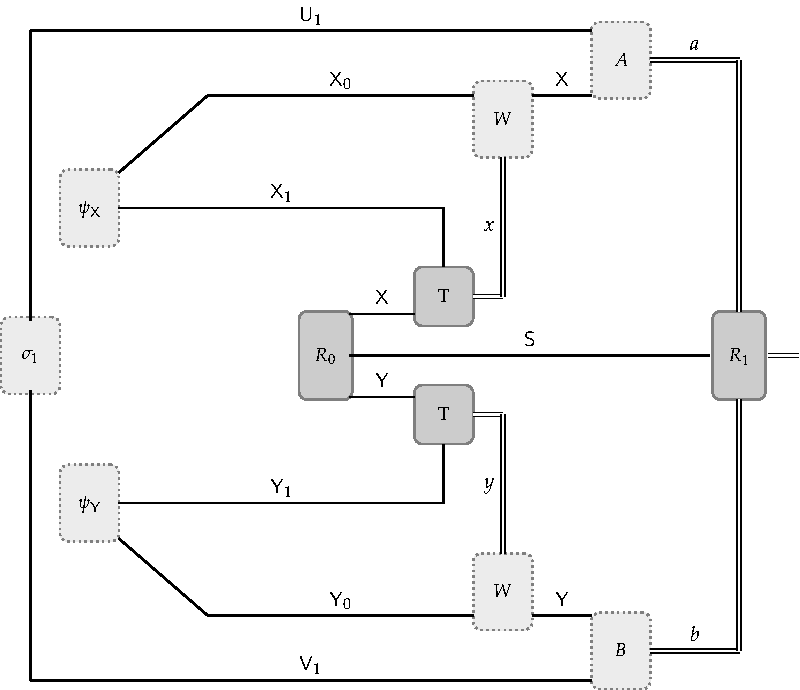
\includegraphics[scale=1.0]{figures/teleportation_game_strategy.pdf}
	\end{center}
		\caption[A teleportation game strategy.]{The strategy that Alice and Bob abide by for a teleportation game when they play honestly. Alice and Bob prepare registers $( \reg{U}_1, \reg{X}_0, \reg{X}_1 )$ and $( \reg{V}_1, \reg{Y}_0, \reg{Y}_1 )$ where register pairs $(\reg{X}_0, \reg{X}_1)$ and $(\reg{Y}_0, \reg{Y}_1)$ consist of pairs of maximally entangled states. The referee receives registers $(\reg{X}_1,\reg{Y}_1)$ and prepares registers $(\reg{X},\reg{S},\reg{Y})$ and performs a measurement in the Bell basis on register pairs $(\reg{X},\reg{X}_1)$ and $(\reg{Y},\reg{Y}_1)$ in order to teleport $\reg{X}$ to Alice and $\reg{Y}$ to Bob. The outcome of these measurements result in $(x,y)$ where $x$ is sent to Alice and $y$ is sent to Bob. Alice and Bob then apply the appropriate Pauli corrections on their registers $\reg{X}_0$ and $\reg{Y}_0$, which teleports the registers $\reg{X}$ and $\reg{Y}$ into their possession. Finally, Alice and Bob respond with answers $a$ and $b$ to the referee, which is followed by the referee performing a measurement $\{Q_{a,b}, \I - Q_{a,b} \} \subset \Pos(\S)$.}
		\label{fig:teleportation-game-strategy}
\end{figure}

Now we show that $\omega_{N}^*(G_t) \leq \omega_{N\abs{\reg{X}}\abs{\reg{Y}}}^*(G_{qc})$. Consider an arbitrary strategy for the teleportation game $G_t$ from above. We show how one may adapt this strategy into a strategy for a quantum-classical game $G_{qc}$. 

Let the referee prepare a quantum state $\rho \in \Density(\X \otimes \S \otimes \Y)$ contained in registers $(\reg{X},\reg{S},\reg{Y})$, and let 
\begin{align}
	\sigma \in \Density( (\U \otimes \X_1) \otimes (\Y_1 \otimes \V) )
\end{align}
be the state shared between Alice, Bob, and the referee contained in registers $(\reg{U},\reg{X}_1,\reg{Y}_1,\reg{V})$. The registers $\reg{X}$ and $\reg{Y}$ are sent to Alice and Bob respectively. Once Alice and Bob receive $\reg{X}$ and $\reg{Y}$, they prepare a two step measurement:

\begin{enumerate}
	\item Alice and Bob measure $(\reg{X},\reg{X}_1)$ and $(\reg{Y},\reg{Y}_1)$ in the Bell basis yielding measurement outcomes 
		\begin{align}
			x \in \SigmaA \quad \textnormal{and} \quad y \in \SigmaB.
		\end{align}
	\item Alice and Bob perform measurements 
		\begin{align}
			\{ A_a^x : a \in \GammaA \} \subset \Pos(\U) \quad \textnormal{and} \quad \{ B_b^y : b \in \GammaB \} \subset \Pos(\V)
		\end{align}
		and obtain respective outcomes $a \in \GammaA$ and $b \in \GammaB$. 
\end{enumerate}
The two-step measurement operators corresponding to outcomes $a$ and $b$ are written as 
\begin{align}
	\sum_{x \in \SigmaA} A_a^x \otimes \phi_x^{\abs{\reg{X}}} \in \Pos(\U \otimes \X_1 \otimes \X) \quad \textnormal{and} \quad \sum_{y \in \SigmaB} B_b^y \otimes \phi_y^{\abs{\reg{Y}}} \in \Pos(\V \otimes \Y_1 \otimes \Y),
\end{align}
where $\phi_x^{\abs{\reg{X}}}$ and $\phi_y^{\abs{\reg{Y}}}$ are Bell measurements. 
%they prepare registers $(\reg{U},\reg{X}_0,\reg{X}_1)$ and $(\reg{V},\reg{Y}_0,\reg{Y}_1)$ respectively such that 
%\begin{align}
%	\abs{\reg{X}_1} = \mA \quad \textnormal{and} \quad \abs{\reg{Y}_1} = \mB.
%\end{align}
%Alice and Bob now measure each pair $(\reg{X},\reg{X}_1)$ and $(\reg{Y},\reg{Y}_1)$ in the Bell basis as in equation~\eqref{eq:bell-basis-telep-game}, yielding strings 
%\begin{align}
%	x = (k_1, k_2) \in \integer_{\mA} \times \integer_{\mA} \quad \textnormal{and} \quad y = (l_1, l_2) \in \integer_{\mB} \times \integer_{\mB}.
%\end{align}
%Alice and Bob respectively apply one of the generalized Pauli operators as in equation~\eqref{eq:gen-pauli-telep} to registers $\reg{X}_0$ and $\reg{Y}_0$. Alice and Bob then produce $a \in \GammaA$ and $b \in \GammaB$ just as they would have done in $G_t$ by performing measurements from the sets 
%\begin{align}
%	\{ A_a : a \in \GammaA\} \subset \Pos(\U \otimes \X) \quad \textnormal{and} \quad \{B_b : b \in \GammaB \} \subset \Pos(\V \otimes \Y).
%\end{align}
Finally, the referee performs a measurement from the set 
\begin{align}
	\{ Q_{a,b}, \I - Q_{a,b} \} \subset \Pos(\S).
\end{align}
It is evident from the above procedure that the information stored in $x \in \SigmaA$ and $y \in \SigmaB$ is precisely what the referee would have sent in $G_t$. Furthermore, the cost of this procedure is given by the dimension of the state $\sigma$, that is
\begin{align}
	N \abs{\reg{X}} \abs{\reg{Y}} = \dim(\U \otimes (\X_1 \otimes \Y_1) \otimes \V).
\end{align}
It then follows that $\omega_{N\abs{\reg{X}}\abs{\reg{Y}}}^*(G_t) \leq \omega_N^*(G_{qc})$.
\end{proof}

%-------------------------------------------------------------------------------
\subsection{Extended nonlocal games and teleportation games} \label{sec:extended-nonlocal-games-and-teleportation-games}
%-------------------------------------------------------------------------------

In the previous section, we established a relationship between certain quantum-classical games and teleportation games. Building on this, we now show how teleportation games and certain extended nonlocal games are related. Once we have this chain of relationships, we will be able to prove Theorem~\ref{thm:enlg-from-qcg}. The following lemma establishes a relationship between teleportation games and extended nonlocal games. 

\begin{lemma} \label{lem:telep-to-enlg}
	Given any teleportation game, $G_t$, with teleported registers $\reg{X}$ and $\reg{Y}$, there exists an extended nonlocal game, $H_t$, such that 
	\begin{align}
		\omega_N^*(H_t) = 1 - \frac{ 1 - \omega_{N}^*(G_t)  }{ \abs{\reg{X}}^2 \abs{\reg{Y}}^2 },
	\end{align}
	for all $N$.
\end{lemma}

In order to prove Lemma~\ref{lem:telep-to-enlg}, as was done previously in the proof of Lemma~\ref{lem:qcg_eq_telep}, we assume that $G_t$ is defined by 
\begin{align}
	\rho \in \Density(\X \otimes \S \otimes \Y) \quad \textnormal{and} \quad \{Q_{a,b} : a \in \GammaA, \ b \in \GammaB \} \subset \Pos(\S).
\end{align} 
We shall also define a specific extended nonlocal game, $H_t$, that consists of a teleportation procedure. From the referee's perspective, such a game is played as follows:
\begin{enumerate}
	\item Alice and Bob present the referee with the register $\reg{R} = (\reg{X}_1, \reg{Y}_1)$ such that 
		\begin{align}
			\abs{\reg{X}_1} = \abs{\reg{X}} \quad \textnormal{and} \quad \abs{\reg{Y}_1} = \abs{\reg{Y}}.
		\end{align}
	Note that the register $\reg{R}$ may be entangled with systems possessed by Alice and Bob, as is the case for ordinary extended nonlocal games. 
	
	\item The referee randomly generates a pair $(x,y) \in \SigmaA \times \SigmaB$ where
	\begin{align}
		\SigmaA = \integer_{\abs{\reg{X}}} \times \integer_{\abs{\reg{X}}} \quad \textnormal{and} \quad \SigmaB = \integer_{\abs{\reg{Y}}} \times \integer_{\abs{\reg{Y}}}	
	\end{align}		
according to the uniform distribution and sends $x \in \SigmaA$ to Alice and $y \in \SigmaB$ to Bob. Alice responds with $a \in \GammaA$ and Bob responds with $b \in \GammaB$. 
	
	\item The referee prepares a state $\rho \in \Density(\X \otimes \S \otimes \Y)$ and then performs a measurement with respect to the binary-valued measurement $\{ P_{a,b,x,y}, \I - P_{a,b,x,y} \}$ where
\begin{equation} \label{eq:ref-meas-telep-enlg}
	\begin{aligned}
		P_{a,b,x,y} &= \I - \phi^{(\abs{\reg{X}})}_{x} \otimes \left( \I - Q_{a,b} \right) \otimes \phi^{(\abs{\reg{Y}})}_y, \\
		\I - P_{a,b,x,y} &= \phi^{(\abs{\reg{X}})}_{x} \otimes \left( \I - Q_{a,b} \right) \otimes \phi^{(\abs{\reg{Y}})}_y, \\
	\end{aligned}	
\end{equation}	 
where $\{Q_{a,b}, \I - Q_{a,b} \} \subset \Pos(\S)$. The outcome corresponding to the measurement $P_{a,b,x,y}$ indicates that Alice and Bob win, while the other measurement indicates that they lose. 
\end{enumerate}
As further intuition for the above protocol, we shall see that the last step may be thought of as a form of \index{post-selected teleportation}{\emph{post-selcted teleportation}} where the randomly selected questions $x$ and $y$ are compared to $x_1$ and $y_1$ which are hypothetical measurement results that would be obtained if the referee were to perform teleportation. Implicit in the winning and losing measurements is the relationship between $(x,y)$ and $(x_1,y_1)$ that
\begin{enumerate}
		\item \emph{If $x \not= x_1$ or $y \not= y_1$}: The referee immediately accepts, and therefore Alice and Bob win. 
		\item \emph{If $x = x_1$ and $y = y_1$}: The referee performs a measurement with respect to the binary-valued measurement $\{Q_{a,b}, \I - Q_{a,b} \}$ on register $\reg{S}$.
	\end{enumerate}
That is, in the event where $x \not= x_1$ or $y \not= y_1$, this corresponds to a failure to teleport $\reg{X}$ or $\reg{Y}$ to Alice or Bob. Likewise, the event where $x = x_1$ and $y = y_1$ corresponds to the event where teleportation protocol would have succeeded, since if the referee \emph{were} to teleport, it would have sent $x_1$ and $y_1$ to Alice and Bob, which would influence the measurement that they would apply to their system. Since in this case $x = x_1$ and $y = y_1$ it is \emph{as if} the referee were to teleport $\reg{X}$ to Alice and $\reg{Y}$ to Bob.

\begin{proof}[Proof of Lemma~\ref{lem:telep-to-enlg}]
Let $H_t$ be the extended nonlocal game as introduced above, and let it be defined in terms of the same state and measurement operators
	\begin{align}
		\rho \in \Density(\X \otimes \S \otimes \Y) \quad \textnormal{and} \quad \{Q_{a,b} : a \in \GammaA \ b \in \GammaB\} \subset \Pos(\S)
	\end{align}
that also define $G_{t}$ such that the measurement operators $\{P_{a,b,x,y}, \I - P_{a,b,x,y}\}$ in $H_t$ are defined in terms of $\{Q_{a,b}, \I - Q_{a,b} \}$ as in equation~\eqref{eq:ref-meas-telep-enlg}. 

Note that in both games $G_t$ and $H_t$, Alice and Bob's strategy is defined by the state
\begin{align}
	\sigma \in \Density(\U \otimes (\X_1 \otimes \Y_1) \otimes \V), \end{align}
as well as their respective measurement operators 
\begin{align}
	\{A_a^x : a \in \GammaA \} \subset \Pos(\U) \quad \textnormal{and} \quad  \{B_b^y : b \in \GammaB \} \subset \Pos(\V).
\end{align}
Let $p$ denote the winning probability for Alice and Bob in $G_t$
\begin{align}
	p = \sum_{\substack{(x,y) \in \SigmaA \times \SigmaB \\ (a,b) \in \GammaA \times \GammaB}} \biggip{ A_a^x \otimes \phi_x^{\abs{\reg{X}}} \otimes Q_{a,b} \otimes \phi_y^{\abs{\reg{Y}}} \otimes B_b^y }{ W (\rho \otimes \sigma) W^* },
\end{align}
where $W$ is the unitary operator that corresponds to the permutation of registers 
\begin{align}
	(\reg{X},\reg{S},\reg{Y},\reg{U},\reg{X}_1,\reg{Y}_1,\reg{V}) \mapsto (\reg{U},\reg{X},\reg{X}_1,\reg{S},\reg{Y},\reg{Y}_1,\reg{V}).
\end{align}
The losing probability for $G_t$ may be derived from the above equation by considering the losing measurement, that is
\begin{align} \label{eq:telep-losing-prob}
	1 - p = \sum_{\substack{(x,y) \in \SigmaA \times \SigmaB \\ (a,b) \in \GammaA \times \GammaB}} \biggip{ A_a^x \otimes \phi_x^{\abs{\reg{X}}} \otimes (\I - Q_{a,b}) \otimes \phi_y^{\abs{\reg{Y}}} \otimes B_b^y }{ W (\rho \otimes \sigma) W^* }.
\end{align}
We will show how the losing probability of $H_t$ may be written in terms of the losing probability of $G_t$. 

Consider an arbitrary strategy for any teleportation game $G_t$. We show how one may adapt this strategy into a strategy for the extended nonlocal game $H_t$. 

Let $(\reg{X}_0, \reg{X}_1)$ and $(\reg{Y}_0,\reg{Y}_1)$ be quantum registers such that
\begin{align}
	 \abs{\reg{X}_0} = \abs{\reg{X}} = \abs{\reg{X}_1} \quad \textnormal{and} \quad  \abs{\reg{Y}_0} = \abs{\reg{Y}} = \abs{\reg{Y}_1},
\end{align}
where the contents of $(\reg{X}_0,\reg{X}_1)$ and $(\reg{Y}_0,\reg{Y}_1)$ are respective maximally entangled states 
\begin{align}
	\psi_{\reg{X}} = \frac{1}{\sqrt{\abs{\reg{X}}}} \sum_{c \in \integer_{\abs{\reg{X}}}} e_c \otimes e_c \quad \textnormal{and} \quad \psi_{\reg{Y}} = \frac{1}{\sqrt{\abs{\reg{Y}}}} \sum_{d \in \integer_{\abs{\reg{Y}}}} e_d \otimes e_d. 
\end{align}
Registers $\reg{X}_1$ and $\reg{Y}_1$ are sent to the referee. 

The referee then chooses $(x,y) \in \SigmaA \times \SigmaB$ at random, according to the uniform probability distribution. The referee makes a local copy of $x$ and $y$ as usual, and then sends $x$ to Alice and $y$ to Bob. Alice and Bob then perform measurements from the sets 
\begin{align}
	\{ A_a^x : a \in \GammaA \} \subset \Pos(\U) \quad \textnormal{and} \quad \{B_b^y : b \in \GammaB \} \subset \Pos(\V),
\end{align}
for each $x \in \SigmaA$ and $y \in \SigmaB$ yielding outcomes $a \in \GammaA$ and $b \in \GammaB$, which are then sent to the referee. 

\begin{figure}[!htpb] 
	\begin{center}
		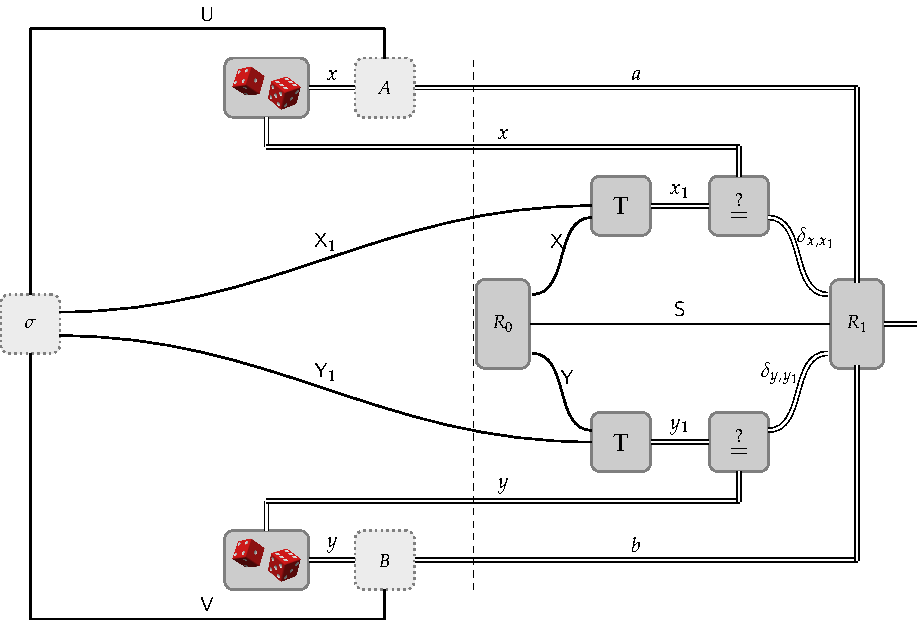
\includegraphics[scale=1.0]{figures/G2.pdf}
	\end{center}
		\caption[The extended nonlocal game $H_t$.]{The extended nonlocal game $H_t$, an extended nonlocal game where the referee initiates a teleportation procedure. That is, once the referee sends questions $(x,y) \in \SigmaA \times \SigmaB$ to Alice and Bob and receives registers $(\reg{X}_1,\reg{Y}_1)$, it shall create a state $\rho \in \Density(\X \otimes \S \otimes \Y)$ in registers $(\reg{X},\reg{S},\reg{Y})$ and perform teleportation using $(\reg{X},\reg{X}_1)$ and $(\reg{Y},\reg{Y}_1)$. The outcome of these teleportation procedures will yield $x_1$ and $y_1$. If both $x_1 = x$ and $y_1 = y$, the referee will perform a measurement on his system, $\reg{S}$, to determine the outcome of the game. Otherwise if $x_1 \not= x$ or $y_1 \not= y$, Alice and Bob automatically win. The dark gray shapes correspond to actions performed by the referee.}
		\label{fig:G2}
\end{figure}

Once the referee receives $a \in \GammaA$ and $b \in \GammaB$, it prepares a state $\rho \in \Density(\X \otimes \S \otimes \Y)$ in registers $(\reg{X},\reg{S},\reg{Y})$ such that 
\begin{align}
	\abs{\reg{X}} = \abs{\reg{X}_1} \quad \textnormal{and} \quad \abs{\reg{Y}} = \abs{\reg{Y}_1}.
\end{align}
The referee now measures $(\reg{X},\reg{X}_1)$ and $(\reg{Y},\reg{Y}_1)$ in the Bell basis, which yields respective outcomes of 
\begin{align}
	x_1 = (k_1,k_2) \in \SigmaA \quad \textnormal{and} \quad y_1 = (l_1,l_2) \in \SigmaB.
\end{align}
We now consider the post-selected teleportation protocol to be a success if $x = x_1$ and $y = y_1$. For each $x_1$ there is a $1/\abs{\reg{X}}^2$ chance that the referee obtains a matching outcome in $x$. Similarly, for each $y_1$, there is a $1/\abs{\reg{Y}}^2$ chance that the referee obtains a matching outcome for $y$. Therefore, the total probability with which the post-selected teleportation protocol is performed successfully is with probability $1/\abs{\reg{X}}^2\abs{\reg{Y}}^2$. 

%Let $\delta_{x,x_1}$ and $\delta_{y,y_1}$ be the Kronecker delta functions defined as 
%\[
% \delta_{x,x_1} =
%  \begin{cases} 
%      \hfill 1 \hfill & \text{ if $x = x_1$}, \\
%      \hfill 0 \hfill & \text{ if $x \not= x_1$} \\
%  \end{cases} 
%  \quad \textnormal{and} \quad 
% \delta_{y,y_1} =
%  \begin{cases} 
%      \hfill 1 \hfill & \text{ if $y = y_1$}, \\
%      \hfill 0 \hfill & \text{ if $y \not= y_1$}. 
%  \end{cases} 
%\] 
Depending on the outcome of the referee's measurement, the game proceeds accordingly:
\begin{enumerate}
	\item If $x \not= x_1$ or $y \not= y_1$, this implies that at least of of the two teleportation protocols has failed. In this case, the referee accepts, and Alice and Bob win the game. 
	\item If $x = x_1$ and $y = y_1$, this implies that both teleportation protocols are successful.
\end{enumerate}
The referee proceeds to perform the measurement $\{P_{a,b,x,y}, \I - P_{a,b,x,y} \}$ defined as in equation~\eqref{eq:ref-meas-telep-enlg}. Let $q$ denote the winning probability of $H_t$
\begin{align}
	q = \frac{1}{\abs{\reg{X}}^2\abs{\reg{Y}}^2} \sum_{\substack{(x,y) \in \SigmaA \times \SigmaB \\ (a,b) \in \GammaA \times \GammaB}} \biggip{A_a^x \otimes P_{x,y,a,b} \otimes B_b^y}{W (\rho \otimes \sigma) W^*},
\end{align}
where again $W$ is the unitary operator that corresponds to the permutation 
\begin{align}
	(\reg{X},\reg{S},\reg{Y},\reg{U},\reg{X}_1,\reg{Y}_1,\reg{V}) \mapsto (\reg{U},\reg{X},\reg{X}_1,\reg{S},\reg{Y},\reg{Y}_1,\reg{V}).
\end{align}
We may write the losing probability of $H_t$ as 
\begin{equation}
	\begin{aligned}
		1-q &= \frac{1}{\abs{\reg{X}}^2\abs{\reg{Y}}^2} \sum_{\substack{(x,y) \in \SigmaA \times \SigmaB \\ (a,b) \in \GammaA \times \GammaB}} \biggip{A_a^x \otimes (\I - P_{x,y,a,b}) \otimes B_b^y}{W (\rho \otimes \sigma) W^*} \\
		&= \frac{1}{\abs{\reg{X}}^2\abs{\reg{Y}}^2} \sum_{\substack{(x,y) \in \SigmaA \times \SigmaB \\ (a,b) \in \GammaA \times \GammaB}} \biggip{A_a^x \otimes \phi_x^{\abs{\reg{X}}} \otimes (\I - Q_{a,b}) \otimes \phi_y^{\abs{\reg{Y}}} \otimes B_b^y}{W (\rho \otimes \sigma) W^*}  \\
		&= \frac{1}{\abs{\reg{X}}^2\abs{\reg{Y}}^2} (1-p).
	\end{aligned}
\end{equation}
Since in both cases we have that $N = \dim(\U \otimes \V)$, optimizing over strategies of cost $N$ gives 
\begin{align}
	\omega_N^*(H_t) = 1 - \frac{ 1 - \omega_N^*(G_t) }{\abs{\reg{X}}^2 \abs{\reg{Y}}^2},
\end{align}
which concludes the proof.

%
%Let us now prove that $\omega_N^*(H_t) \leq 1 - \frac{1 - \omega_{N\mA\mB}^*(G_t)}{\abs{\reg{X}}^2 \abs{\reg{Y}}^2}$. Consider an arbitrary strategy for any extended nonlocal game, $H_t$. We show how one may adapt this strategy into a strategy for a teleportation game $G_t$. 
%
%Alice and Bob prepare registers $(\reg{U},\reg{X}_1)$ and $(\reg{V},\reg{Y}_1)$ and send $\reg{X}_1$ and $\reg{Y}_1$ to the referee. When the referee receives $\reg{X}_1$ and $\reg{Y}_1$, it prepares a state $\rho \in \Density(\X \otimes \S \otimes \Y)$ in registers $(\reg{X},\reg{S},\reg{Y})$ where
%\begin{align}
%	\abs{\reg{X}} = \mA = \abs{\reg{X}_1} \quad \textnormal{and} \quad \abs{\reg{Y}} = \mB = \abs{\reg{Y}_1},
%\end{align} 
%along with $(x,y) \in \SigmaA \times \SigmaB$, which are chosen according to the uniform probability distribution. The referee then performs a measurement in the Bell basis on registers $(\reg{X},\reg{X}_1)$ and $(\reg{Y},\reg{Y}_1)$ that yield outcomes 
%\begin{align}
%	x_1 = (k_1,k_2) \in \integer_{\mA} \times \integer_{\mA} \quad \textnormal{and} \quad y_1 = (l_1,l_2) \in \integer_{\mB} \times \integer_{\mB}.
%\end{align}
%The referee makes a local copy of $(x,y)$ and then sends $x$ to Alice and $y$ to Bob. Alice and Bob then compute $a \in \GammaA$ and $b \in \GammaB$ by performing measurements 
%\begin{align}
%	\{A_a^x : a \in \GammaA \} \subset \Pos(\U) \quad \textnormal{and} \quad \{B_b^y : b \in \GammaB \} \subset \Pos(\V),
%\end{align}
%for each $x \in \SigmaA$ and $y \in \SigmaB$, and sends the results $a \in \GammaA$ and $b \in \GammaB$ to the referee. When the referee receives $a$ and $b$, it checks $(x,y)$ against $(x_1,y_1)$. If it happens that $x = x_1$ and $y = y_1$, it accepts and Alice and Bob win the game. This outcome is akin to the teleportation procedure succeeding in $H_t$. This occurs with a $1/\mA^2 \mB^2$ probability. Otherwise, the referee performs a measurement $\{Q_{a,b}, \I - Q_{a,b}\} \subset \Pos(\S)$ on register $\reg{S}$. It is evident that the probability with which the strings $x = x_1$ and $y = y_1$ occur with the same probabilities as they do in $H_t$. It therefore stands that $\omega_N^*(H_t) \leq 1 - \frac{1 - \omega_{N\mA\mB}^*(G_t)}{\abs{\reg{X}}^2 \abs{\reg{Y}}^2}$. 

\end{proof}


%-------------------------------------------------------------------------------
\subsubsection*{Proof of Theorem~\ref{thm:enlg-from-qcg}}
%-------------------------------------------------------------------------------

\begin{proof}[Proof of Theorem~\ref{thm:enlg-from-qcg}]
	Recall from Lemma~\ref{lem:qcg_eq_telep} we have that 
	\begin{align}
		\omega_N^*(G_{qc}) \leq \omega_{N\abs{\reg{X}}\abs{\reg{Y}}}^*(G_t) \quad \textnormal{and} \quad \omega^*_{N}(G_t) \leq \omega^*_{N\abs{\reg{X}}\abs{\reg{Y}}}(G_{qc}),
	\end{align}		
	for all $N \geq 1$. From Lemma~\ref{lem:telep-to-enlg} it follows that 
	\begin{align}
		1 - \frac{1 - \omega_{N}^*(G_t)}{\abs{\reg{X}}^2\abs{\reg{Y}}^2} = \omega_N^*(H_t).
	\end{align}
	It then follows that the inequalities from equation~\eqref{eq:enlg-from-qcg} hold.
	%\begin{align}
%		\omega^*(H_t) = 1 - \frac{1-\omega^*(G_{qc})}{\abs{\reg{X}}^2\abs{\reg{Y}}^2}.
%	\end{align}
	Furthermore, it follows from Theorem~\ref{thm:regev-vidick-qcg} that there exists a quantum-classical game $G_{qc}$ where $\omega_N^*(G_{qc}) = 1$ is achieved in the limit as $N$ goes to infinity. It then follows that there also exists an extended nonlocal game $H_t$, where $\omega_N^*(H_t) = 1$ as $N$ approaches infinity. 
\end{proof}

%-------------------------------------------------------------------------------
\subsubsection*{Implications and discussion of Theorem~\ref{thm:enlg-from-qcg}}
%-------------------------------------------------------------------------------

We briefly discuss the broader context of Theorem~\ref{thm:enlg-from-qcg}. As previously mentioned, Regev and Vidick~\cite{Regev2013} proved that a certain class of QC games have the property that if Alice and Bob make use of an entangled state initially shared between them, they can never achieve perfect optimality, it is always possible for them to do better (meaning that they win with a strictly larger probability) using some different shared entangled state on larger quantum systems. We found in the previous section that there also exists a class of extended nonlocal games with this property as well. 
 
We can also ask whether or not the above property holds more generally for some class of nonlocal games. Formally, 
\begin{question}
	Does there exist a nonlocal game $G$ such that 
	\begin{align}
		\omega^*(G) = 1,
	\end{align}
	and for every positive integer $N$ it holds that 
	\begin{align}
		\omega_N^*(G) < 1.
	\end{align}
\end{question}
For the traditional nonlocal game case with classical questions and classical answers, this question remains open. The so-called \index{I3322 inequality}{\emph{I3322 inequality}}, when formulated as a nonlocal game, has been conjectured to have the property just described, in which increasing degrees of entanglement admit strategies with strictly increasing success rates~\cite{Pal2009}.

It is also worth noting that Theorem~\ref{thm:enlg-from-qcg} implies the existence of a tripartite steering inequality for which an infinite-dimensional quantum state is required in order to achieve a maximal violation. This follows from the fact that extended nonlocal games may be equivalently viewed as a tripartite steering scenario (as considered in~\cite{Cavalcanti2015} and~\cite{Sainz2015}), as was mentioned in Chapter~\ref{chap:extended_nonlocal_games}. 

%%-------------------------------------------------------------------------------
%\subsection{Extended nonlocal games and tripartite steering} 
%%-------------------------------------------------------------------
%
%\index{quantum steering}{\emph{Quantum steering}}, first introduced by Schr{\"o}dinger~\cite{Schroedinger1935}, refers to a scenario in which Alice and Bob share an unknown state and the actions of Alice performing a measurement on her local subsystem of the shared state results in a change in the local subsystem held be Bob. Since this scenario occurs between two parties, we refer to this steering scenario as \index{bipartite steering}{\emph{bipartite steering}}. In such a scenario, we are provided with a full description of the measurement operators used by Bob, but no description of Alice's measurement operators is assumed. Alice's goal is to perform an appropriate sequence of measurements to her subsystem in such a way to convince Bob that the state that they share is entangled. That is, Alice's goal is to ``\emph{steer}'' the state on Bob's portion of the shared state by performing measurements on her subsystem to convince Bob that the shared state is entangled. 
%
%More formally, a bipartite steering scenario is characterized by alphabets, $\SigmaA$ and $\GammaA$. Alice and Bob share an unknown bipartite state, $\rho \in \Density(\A \otimes \B)$, where $\A$ and $\B$ refer to the respective complex Euclidean spaces belonging to Alice and Bob. Alice is equipped with a set of unknown measurement operators 
%\begin{align}
%	\{A_a^x : a \in \Gamma \} \subset \Pos(\A),
%\end{align}
%for each $x \in \SigmaA$ such that 
%\begin{align}
%	\sum_{a \in \GammaA} A_a^x = \I_{\A}. 
%\end{align}
%When analyzing a bipartite steering scenario, it may be convenient to define a function $K : \GammaA \times \SigmaA \rightarrow \Pos(\B)$ as 
%\begin{align}
%	K(a|x) = \tr_{\A} \left( \left(A_a^x \otimes \I_{\B} \right) \rho \right)
%\end{align}
%for each $a \in \GammaA$ and $x \in \SigmaA$. We call the function $K$ a \index{bipartite steering assemblage}{\emph{bipartite steering assemblage}}. The operators output by this function represent unnormalized states of Bob's quantum system when Alice outputs $a$ for an input $x$. Assuming that $\tr(K(a|b)) > 0$, we can normalize the states from function $K$ as 
%\begin{align}
%	\rho_a^x = \frac{K(a|b)}{\tr(K(a|b)}.
%\end{align}
%This function completely characterizes the performance of Alice since it encodes the probability that Alice obtains outcome $a \in \GammaA$ given $x \in \SigmaA$. 
%
%The steering scenario may be extended to the setting of three participants. This setting is referred to as \index{tripartite steering}{\emph{tripartite steering}}. Indeed, the notion of extended nonlocal games generalize a particular type of \emph{tripartite steering}, that is, a steering scenario consisting of three parties where two of the parties (Alice and Bob) are untrusted. In the steering literature, this type of steering scenario is sometimes referred to as a \index{tripartite two-sided device independent scenario (see also tripartite steering, extended nonlocal game)}{\emph{tripartite two-sided device independent scenario}}, but we shall refer to it as just \index{tripartite steering with two untrusted parties}{\emph{tripartite steering with two untrusted parties}}. Tripartite and multipartite steering scenarios were investigated in~\cite{Cavalcanti2015} and~\cite{Sainz2015}.
%
%Given this connection between extended nonlocal games and tripartite steering scenarios with two untrusted parties, we consider what the implication of Theorem~\ref{thm:enlg-infinite-ent} is for tripartite steering. 
%
%\comment{This is where it would make sense to elaborate on how the previously mentioned result can be interpreted in terms of steering inequalities. Some of this may be contingent on how the result is presented when it is written up in paper form.}


%-------------------------------------------------------------------------------
\section{Variations on the extended nonlocal game model} \label{sec:variations-on-enlg}
%-------------------------------------------------------------------

Recall that a nonlocal game consists of two rounds of communication: one from the referee to the players and one from the players to the referee. The standard definition of a nonlocal game assumes that both rounds of communication consist of classical messages. We saw a variation on that model in Section~\ref{sec:quantum-classical-games}, in which the question round was replaced with the referee sending quantum questions to both Alice and Bob. In a similar manner, we may also consider such variations on the extended nonlocal game model. The standard extended nonlocal game consists of three rounds of communication, that is
\begin{enumerate}
	\item (Quantum): Alice and Bob prepare a state $\sigma \in \Density(\U \otimes \R \otimes \V)$ shared between themselves and the referee. 
	\item (Classical): The referee randomly generates classical questions for Alice and Bob, $(x,y) \in \SigmaA \times \SigmaB$, respectively.
	\item (Classical): Alice and Bob respond with answers $a \in \GammaA$ and $b \in \GammaB$. 
\end{enumerate}
In complete generality, any variation on the type of communication used in an extended nonlocal game may be specified in terms of a tuple $(t_1,t_2,t_3) \in \{q,c\}$ where each round of communication consists of either a transmission of classical or quantum information as denoted by either $c$ or $q$ in the tuple. For instance, the type of communication in each round of a standard extended nonlocal game corresponds to the tuple $(q,c,c)$. We therefore equivalently may refer to the standard definition of an extended nonlocal game as a quantum-classical-classical extended nonlocal game or just a QCC extended nonlocal game for short. 

%For convenience, we may refer to the class of extended nonlocal games equivalently as ${\bf H}_{qcc}$ to be explicit about the form of communication for each round. In complete generality, we define ${\bf H}_{t_1 t_2 t_3}$ with $t_1,t_2,t_3 \in \{q,c\}$ to be a class of extended nonlocal game where each round of communication may either consist of classical or quantum communication. 

%-------------------------------------------------------------------------------
\subsection{Quantum-classical-quantum extended nonlocal games}
%-------------------------------------------------------------------------------

Consider the class of \index{quantum-classical-quantum extended nonlocal games}{\emph{quantum-classical-quantum extended nonlocal games}} or QCQ extended nonlocal games for short. This class of game is defined precisely as a standard extended nonlocal game, only now the last round of communication is replaced with Alice and Bob sending quantum registers in place of the classical message $a \in \GammaA$ and $b \in \GammaB$ to the referee. 

Specifically, a QCQ extended nonlocal game is specified by the following objects:
\begin{itemize}
	\item A probability distribution $\pi : \SigmaA \times \SigmaB \rightarrow [0,1]$, for alphabets $\SigmaA$ and $\SigmaB$. 
	\item A collection of measurement operators $\{P_{x,y} : x \in \SigmaA, \ y \in \SigmaB \} \subset \Pos(\A \otimes \R \otimes \B)$ where $\A,\B$, and $\R$ are complex Euclidean spaces corresponding to registers $\reg{A},\reg{B},$ and $\reg{R}$. 
\end{itemize}
From the referee's perspective, such a game is played as follows: 
\begin{enumerate}
	\item Alice and Bob present the referee with the register $\reg{R}$, which has been initialized in a state of Alice and Bob's choosing. (The register $\reg{R}$ might, for instance, be entangled with systems possessed by Alice and Bob.)
	\item The referee randomly generates a pair $(x,y) \in \SigmaA \times \SigmaB$ according to the distribution $\pi$, and sends $x$ to Alice and $y$ to Bob. Alice and Bob then send registers $\reg{A}$ and $\reg{B}$ corresponding to spaces $\A$ and $\B$ to the referee. 
	\item The referee measures registers $(\reg{A},\reg{R},\reg{B})$ with respect to the binary-valued measurement $\{P_{x,y}, \I - P_{x,y}\} \subset \Pos(\A \otimes \R \otimes \B)$. The outcome corresponding to the measurement operator $P_{x,y}$ indicates that Alice and Bob win, while the other measurement result indicates that they lose. 
\end{enumerate}
For any QCQ extended nonlocal game, there are various classes of strategies that may be adapted from the standard extended nonlocal game case for Alice and Bob, including unentangled strategies, standard quantum strategies, commuting measurement strategies, and non-signaling strategies. In this section, we only consider standard quantum strategies for QCQ extended nonlocal games.

A standard quantum strategy for a QCQ extended nonlocal game, specified by 
\begin{align}
	\pi : \SigmaA \times \SigmaB \rightarrow [0,1] \quad \textnormal{and} \quad \{P_{x,y} : x \in \SigmaA, \ y \in \SigmaB \} \subset \Pos(\A \otimes \R \otimes \B)
\end{align}
as above, consists of these objects: 

\begin{enumerate}
	\item A state $\sigma \in \Density(\U \otimes \R \otimes \V)$, for $\U$ being the space corresponding to a register $\reg{U}$ held by Alice and $\V$ being the space corresponding to a register $\reg{V}$ held by Bob. This state represents Alice and Bob's initialization of the tripe $(\reg{U},\reg{R},\reg{V})$ immediately before $\reg{R}$ is sent to the referee. 
	\item A collection of channels $\{ \Phi^x \} \subset \Channel(\U,\A)$ for each $x \in \SigmaA$, applied by Alice when she receives the question $x$, and a collection of channels $\{\Phi^y \} \subset \Channel(\V,\B)$ for each $y \in \SigmaB$, applied by Bob when he receives the question $y$. Alice and Bob then send their portions of the state after they have applied their channels to the referee. 
\end{enumerate} 
When Alice and Bob utilize such a strategy, their winning probability may be expressed as 
\begin{align}
	  \sum_{\substack{
      (x,y) \in \SigmaA \times \SigmaB 
  }}
	\biggip{P_{x,y}}{ \left( \Phi^x \otimes \I_{\Lin(\R)} \otimes \Phi^y \right) \left(\sigma\right) }.
\end{align}
\begin{figure}[!htpb] 
	\begin{center}
			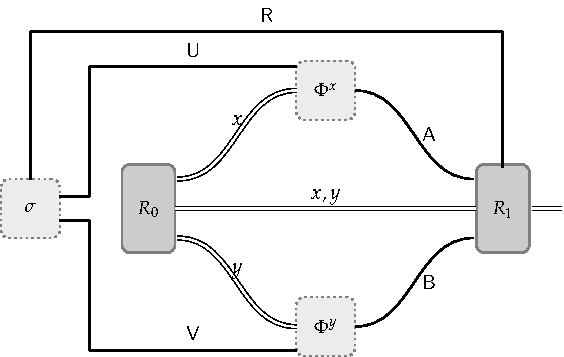
\includegraphics[scale=1.0]{figures/qcq_enlg.pdf}
	\end{center}
		\caption[A quantum-classical-quantum extended nonlocal game.]{A quantum-classical-quantum extended nonlocal game. The referee selects questions $(x,y) \in \SigmaA \times \SigmaB$ according to the probability distribution $\pi$, and sends $x$ to Alice and $y$ to Bob. Upon receiving $(x,y)$, Alice and Bob apply channels $\Phi^x$ and $\Phi^y$ to their respective systems and respond with answers in the form of quantum registers $(\reg{A},\reg{B})$ over complex Euclidean spaces $\A$ and $\B$. After receiving $(\reg{A},\reg{B})$ from Alice and Bob, the referee performs a measurement on $\{P_{x,y}, \I - P_{x,y}\}\subset \Pos(\A \otimes \R \otimes \B)$ to determine the probability with which Alice and Bob win or lose.}
		\label{fig:quantum-classical-quantum-enlg}
\end{figure}
Using a similar teleportation trick that we have used in Section~\ref{sec:extended-nonlocal-games-and-teleportation-games}, one may show that an arbitrary strategy for a QCC extended nonlocal game may be adapted for a QCQ extended nonlocal game. There is not much to be gained from going through the explicit details of this, as they are nearly identical to the process we have seen in the section already.

It is, however, relevant to note that in Lemma 32 of~\cite{Kobayashi2015}, the authors use a similar teleportation trick to prove a relationship between two different subclasses of complexity classes arising from what they refer to as the ``generalized-QAM'' complexity class. These two subclasses are similar in some sense to the QCC extended nonlocal game model and the QCQ extended nonlocal game model, as the authors also analyze variants of the QAM complexity class with similar properties.  

%%-------------------------------------------------------------------------------
%\subsubsection*{Quantum-classical-quantum extended nonlocal games and extended nonlocal games}
%%-------------------------------------------------------------------------------
%
%The following theorem states that Alice and Bob gain no advantage in playing any quantum-classical-quantum extended nonlocal game over a standard extended nonlocal game. 
%
%\begin{lemma} \label{lem:qcc-eq-qcq}
%For any extended nonlocal game $H_{qcc}$ and any quantum-classical-quantum extended nonlocal game $H_{qcq}$, it holds that
%	\begin{align}
%		\omega^*(H_{qcc}) = \omega^*(H_{qcq}).
%	\end{align}
%\end{lemma}
%
%As part of the proof of Lemma~\ref{lem:qcc-eq-qcq}, we are going to define a specific extended nonlocal game, $H_{qcc-t}$, that consists of a teleportation procedure and is depicted in Figure~\ref{fig:enltg}.
%\begin{enumerate}
%	\item Alice and Bob present the referee with the register $\reg{R} = (\reg{X}_1,\reg{Y}_1)$, which has been initialized in a state of Alice and Bob's choosing. The register $\reg{R}$ may be entangled with systems possessed by Alice and Bob. 
%	\item The referee randomly generates a pair $(x,y) \in \SigmaA \times \SigmaB$ according to the distribution $\pi$, and then sends $x$ to Alice and $y$ to Bob. Alice creates $\rho_{\reg{A}} \in \Density(\A)$ contained in register $\reg{A}$ and Bob creates $\rho_{\reg{B}} \in \Density(\B)$ contained in register $\reg{B}$.  
%	\item Alice and Bob take part in a teleportation protocol with the referee, where the outcome of the respective protocols are sent to the referee, where it completes the teleportation procedure and performs a measurement on $\reg{R}$. 
%\end{enumerate}
%
%\begin{figure}[!htpb] 
%	\begin{center}
%			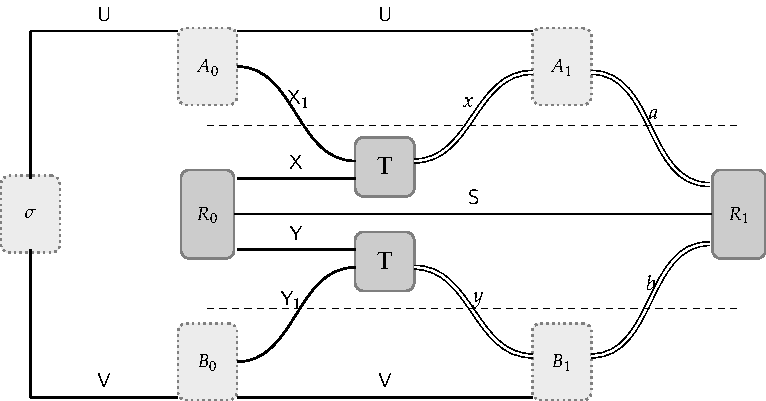
\includegraphics[scale=1.0]{figures/qcc_teleport.pdf}
%	\end{center}
%		\caption[The $H_{qcc-t}$ game.]{The $H_{qcc-t}$ game. }
%\label{fig:enltg}		
%\end{figure}
%
%\begin{proof}[Proof of Lemma~\ref{lem:qcc-eq-qcq}]
%	It is evident that $\omega^*(H_{qcc}) \leq \omega^*(H_{qcq})$ for every standard extended nonlocal game and for every quantum-classical-quantum extended nonlocal game since the referee could have just as well measured the states provided by Alice and Bob in the last round, and used the classical outcome for the final measurement. 
%
%To show $\omega^*(H_{qcq}) \leq \omega^*(H_{qcc})$, the primary idea is to show that we can adapt any strategy for a quantum-classical-quantum extended nonlocal game for an extended nonlocal game $H_{qcc-t}$ as previously defined and depicted in Figure~\ref{fig:enltg}. The approach to prove this direction is similar to the technique used in the proof of Lemma 32 of~\cite{Kobayashi2015}. 
%
%%\comment{Question: How do $P^{x,y}$ and $P^{a,b}$ relate?}
%
%\comment{Not sure how to define these measurements for the $H_{qcq}$ game.}
%
%Let $H_{qcc-t}$ be the extended nonlocal game, as introduced above, and let it be defined in terms of the same probability distribution $\pi$ and collection of measurement operators $\{ \}$ that also define $H_{qcq}$ where 
%\begin{align}
%	P_{a,b,x,y} = \tr_{\A \otimes \B}(P_{x,y}) \quad \textnormal{and} \quad \I - P_{a,b,x,y} = \I - \tr_{\A \otimes \B}(P_{x,y}).
%\end{align}
%
%Let us prove that $\omega^*(H_{qcq}) \leq \omega^*(H_{qcc-t})$. Consider an arbitrary strategy for any quantum-classical-quantum extended nonlocal game, $H_{qcq}$. We show how one may adapt this strategy into a strategy for the extended nonlocal game $H^{\prime}_{qcc}$. Let Alice and Bob prepare quantum registers $(\reg{U},\reg{X}_1, \reg{A})$ and $(\reg{V},\reg{Y}_1, \reg{B})$, respectively, such that 
%\begin{align}
%	\abs{\reg{U}} = \mA = \abs{\reg{X}_1}, \quad \abs{\reg{V}} = \mB = \abs{\reg{Y}_1}, \quad \abs{\reg{A}} = 2 \mA, \quad \textnormal{and} \quad \abs{\reg{B}} = 2 \mB,
%\end{align}
%where the contents of $(\reg{U},\reg{X}_1)$ and $(\reg{V},\reg{Y}_1)$ are respective maximally entangled states defined as 
%\begin{align}
%	\frac{1}{\sqrt{\mA}} \sum_{c \in \integer_{\mA}} e_c \otimes e_c \quad \textnormal{and} \quad \frac{1}{\sqrt{\mB}} \sum_{d \in \integer_{\mB}} e_d \otimes e_d
%\end{align}
%
%Once the referee receives the registers $\reg{X}_1$ and $\reg{Y}_1$ from Alice and Bob, it randomly generates $(x,y) \in \Sigma$ according to the probability distribution $\pi$. Alice and Bob receive $x \in \SigmaA$ and $y \in \SigmaB$ respectively and perform respective measurements on $(\reg{U}, \reg{A})$ and $(\reg{V},\reg{B})$ in the Bell basis 
%\begin{align} \label{eq:bell-basis-infinite}
%	\left \{ \phi^{(\mA)}_{k_1, k_2} : k_1, k_2 \in \integer_{\mA} \right \} \quad \textnormal{and} \quad \left \{ \phi^{(\mB)}_{l_1, l_2} : l_1, l_2 \in \integer_{\mB} \right \}.
%\end{align}
%The outcomes of performing these measurements for Alice and Bob are 
%\begin{align}
%	a = (k_1, k_2) \in \integer_{\mA} \times \integer_{\mA} \quad \textnormal{and} \quad b = (l_1, l_2) \in \integer_{\mB} \times \integer_{\mB}.
%\end{align}
%Then, Alice and Bob send $a \in \GammaA$ and $b \in \GammaB$ respectively to the referee. The referee applies the appropriate generalized Pauli operators
%\begin{align} \label{eq:gen-pauli-ops-inf}
%	\left \{ W_{k_1,k_2}^{(\mA)} = X_{\mA}^{k_1} Z_{\mA}^{k_2} : k_1,k_2 \in \integer_{\mA} \right \} \quad \textnormal{and} \quad \left \{ W_{l_1,l_2}^{(\mB)} = X_{\mB}^{l_1} Z_{\mB}^{l_2} : l_1,l_2 \in \integer_{\mB} \right \},
%\end{align}
%to his registers $\reg{X}_1$ and $\reg{Y}_1$ respectively to complete the teleportation procedure. This action effectively teleports the registers $\reg{A}$ and $\reg{B}$ from Alice and Bob to the referee. It is then evident that the referee must also accept with at least the same probability as in $H_{qcc-t}$. It follows that $\omega^*(H_{qcq}) \leq \omega^*(H_{qcc-t})$. 
%
%Let us now prove that $\omega^*(H_{qcc-t}) \leq \omega^*(H_{qcq})$. Consider an arbitrary strategy for any extended nonlocal game of the form, $H_{qcc-t}$. We show how one may adapt this strategy into a strategy for a quantum-classical-quantum extended nonlocal game. Let Alice and Bob prepare registers $(\reg{X}_1, \reg{A}, \reg{U})$ and $(\reg{Y}_1, \reg{B}, \reg{V})$ such that 
%\begin{align}
%	\abs{\reg{A}} = \mA = \abs{\reg{X}_1} \quad \textnormal{and} \quad \abs{\reg{B}} = \mB = \abs{\reg{Y}_1}.
%\end{align}
%Alice and Bob then send $\reg{X}_1$ and $\reg{Y}_1$ to the referee. The referee then randomly generates and sends $(x,y) \in \Sigma$ according to the distribution $\pi$. 
%
%Alice and Bob then take part in the following procedure to teleport the registers $\reg{A}$ and $\reg{B}$ to themselves. Alice and Bob apply a measurement to their registers $(\reg{U})$ and $(\reg{V})$ in the Bell basis as from equation~\eqref{eq:bell-basis-infinite}. The respective outcomes of performing this measurement are $a \in \GammaA$ and $b \in \GammaB$ where 
%\begin{align}
%	a = (k_1, k_2) \in \integer_{\mA} \times \integer_{\mA} \quad \textnormal{and} \quad b = (l_1, l_2) \in \integer_{\mB} \times \integer_{\mB},
%\end{align}
%are used to apply respective generalized Pauli operators as from equation~\eqref{eq:gen-pauli-ops-inf} to their respective registers $\reg{A}$ and $\reg{B}$.
%
%Alice and Bob then send $\reg{A}$ and $\reg{B}$ to the referee. From this construction, it is evident that the probability in which the referee accepts is at least as much as in $H_{qcc-t}$. Hence the direction $\omega^*(H_{qcq}) \leq \omega^*(H_{qcc-t})$ is shown. 
%\end{proof}
%
%
%%\subsection{Classical-quantum-classical extended nonlocal games}
%%
%%\comment{TODO : CQC $\leq$ QCC}
